\chapter{Conclusion}\label{Chap:Conclusion}

This final chapter will conclude this bachelor's thesis. After summarising the project and its biggest components, I will propose some solutions to solve the evaluated problems from section~\ref{Chap:Evaluation}. After that, a section about a possible technology transfer will follow, which describes how the PARRHI system could be fitted to other hardware (robots, factory machines, AR devices), programming languages or also 3D game engines. The very last section outlines some future projects, which could build upon this bachelor's thesis.

\section{Summary}

Developing Augmented Reality applications needs a certain set of skills, which involves knowledge in different frameworks, programming languages and engines. In the industry professionals of their field often do not have any experience with AR development, which either results in no applications being developed, or Software Engineers being hired, which increases communication efforts, costs and possibly the time to market. 

The presented system called "PARRHI" (Parametrised Augmented Reality Robot Human Interface) tries to solve the problem of interdisciplinarity by enabling people, who do not have any skills towards AR development or programming in general, to quickly and easily develop and execute AR applications for their specific domain. 

The approach is, to create an abstract layer above all technicalities, that handle the Augmented Reality and real world communication components. The developer, which is the person with the specific domain knowledge, who wants to create such an AR application, now can focus on the application's workflow, and let the PARRHI system manage all other aspects like image tracking, AR, wireless communication with the real world and more.

To further support the developer, the PARRHI system follows a concept called "parametric thinking". This means, that the program, which is written by the developer, is parametrised using placeholders. These placeholders can now be data which the PARRHI system discloses to the program, or also other objects defined in the parametrised program. 

In conclusion, the developer's necessary skill set is limited to their specific domain knowledge. The PARRHI system handles all other aspects of AR Human Robot Interfaces on its own.

\section{Solution to Problems found in Evaluation}\label{Section:SolutionToEval}

The evaluation (see chapter~\ref{Chap:Evaluation}) found two major flaws in the current concept of the PARRHI system. Firstly, the expermimentees lost the overview of their own parametrised program. Secondly, the possible use cases are limited by PARRHI's predefined capabilities.

\subsection{Solution to Problem 1: Overview and Program Complexity}
This problem might be solvable in two distinct but not exclusive ways.

The discussion with the experimentees from evaluation 2 brought up, that a simple re-organisation of the parametrised program's structure could help to increase the overview. Namely, the separation of triggers and their corresponding actions in combination with the name referencing confused the developers, when their program grew in length.

By allowing actions and triggers to be defined underneath the same XML-parent element, the logical workflow could be represented in the program much better. Furthermore, adding the possibility to define "inline actions" would help to reduce the number of names (and with that the confusion) within a program.

Most of the time, one action was exclusively triggered by one trigger. This one to one relation, could be referenced implicitly by defining the action as xml-children of the trigger. As showed in the example below. A trigger would then invoke all implicitly referenced actions in addition to the ones defined with the \code{actions} parameter.

These implicitly referenced actions do not need a name parameter, since their execution is defined by their parent trigger.

\begin{lstlisting}
<!-- Define Trigger -->
<DistanceTrigger name="DTrigger" point1="..." point2="..." distance="15" actions="...">
	<!-- Define Action -->
	<ChangeUITextAction text="You have reached your target successfully!"/>
</DistanceTrigger>
\end{lstlisting}

Another possible solution to reduce the confusion and complexity within the parametrised program would be a graphical editor, which generates the xml document. The syntax defined in the parametrised program is an almost perfect fit for UML activity diagrams (for reference, see Fig.~\ref{Fig:Evaluation2Workflow}.). A more thorough explanation of such an editor is defined in section~\ref{Section:FutureWork}.

\subsection{Solution to Problem 2: PARRHI's Limitations}

With the PARRHI system the developer can only perform actions, which are directly supported by the different types of actions. Whenever an action, which is not available in the PARRHI system, should be performed, the system reaches its limits. The same is true, if the application should display holograms in different shapes than spheres and cylinders.

This problem could be surpassed by allowing the developer to define custom implementations of certain components within the parametrised program. In the simplest case, this implementation could be provided in a specific $C\#$ source code file. The developer would get access to all parameters provided by the PARRHI system, and would also be able to reference objects defined within the parametrised program.

This way, the developer could setup and solve the simple parts within the parametrised program with the supplied object types, and implement everything else on his own. For example, if the developer needs a very specific trigger to be defined, they could achieve that, by directly implementing them in source code. The developer would still not care about any AR functionalities and can still focus on his domain knowledge. 

The defined custom components could then be used in the parametrised program as any other type of trigger, provided they are implemented with the correct properties. 

The actual usage could work in such a way, that developers continuously extend their custom implementations, and use them like normal elements in the parametrised program. In larger companies, one software engineer could take over the task of implementing these specific functionalities, and less skilled or specialised developers could use these custom elements in their parametrised program.


\section{Technology Transfer}\label{Section:TechnologyTransfer}

This section will describe what measurements had to be undertaken, in order to extend the PARRHI system as it is, for a wider variety of use cases and functionalities. The structure of this section will be grouped by technologies or components within the PARRHI implementation.

\subsection{Replacing the Target Machine}
In the provided implementation a Fanuc CR-7iA/L robot was chosen as a demonstrator for the PARRHI concept. Of course there is a big variety of desirable targetable machines, like other robot types from Fanuc or other suppliers, other machines like industry 4.0 machines etc.

The PARRHI library is written in a very modular manner. This means, that extending or replacing certain parts of it is very easy. To replace the target machine, one would only have to extend the Input/Output modules and the Real World Model, to be able to communicate with the desired machine.

At this point, I have to separate three different cases. Case 1 would be to communicate with another robot in the Fanuc product family. Case 2 is to communicate with an industrial robot of another brand and finally case 3 would be to include machines which are not industrial robots. 

Case 1 is very easily achievable, since we built a working communication system for Fanuc controllers. In this case, only the Real World Model has to be updated, since the forward kinematics is based on this specific robot. The modification to involve other Fanuc robots would thereby only mean, to adapt the forward kinematic model's vectors and matrices as defined in section~\ref{Section:ForwardKinematics}. Currently, this model is defined in source code, since in my specific implementation example I only had one robot to work with. So a generalisation would have been a slight overkill. Theoretically, one could simply expose the forward kinematics model via an Interface, and let knowledgable developers implement their own robot. 

Case 2 is a bit more tricky, since the communication problem has to be solved again. One could reuse the Robot Library (see section~\ref{Section:RobotLibrary}), and only replace the other endpoint of the network socket with the new robot. Of course the actual controlling and parsing of the commands on the robot side, would have to be rewritten on the specific system. Our current KAREL / TP solution only works on Fanuc Robot-Controllers and not on any other type of industrial robot. Then again the forward kinematic's model would need an adaption to the new robot too.

Case 1 and Case 2 do not require any changes to the PARRHI system itself. The Parametrised Program could be used as it is. In case 3 though, this would likely change, since conceptually another machine is not the same as an industrial robot. The Distance Trigger for example would not make any sense, if the target machine does not have any moving parts. This means, that in addition to the communication module (Input / Output Modules), one would probably have to define new triggers and actions for the target machine, what requires changes to the PARRHI library itself. Since the PARRHI library is implemented with element base classes and inheritance structures, the implementation of custom triggers and actions is rather easy.

\subsection{Replacing the AR / 3D Engine}

The current implementation is uses the Unity Game Engine as a host. Since all the application logic (PARRHI Library) and also the Robot Library is implemented in engine independent .NET libraries, one could easily switch to any other 3D engine, which is capable of building for Augmented Reality Devices, and is able to include .NET dynamically linked libraries (DLLs). 

The new implementation would have to implement three main aspects: Firstly, the engine has to host the PARRHI and Robot libraries, which is easy, as long as the engine's scripting environment supports .NET libraries. Sencondly, the AR-Output Module has to be rewritten for the new engine. In my implementation, this only took about 30 lines of code. The AR-Output module only instantiates new Holograms in the engine's environment and displays them accordingly. Lastly, the image tracking problem would have had to be solved again. The used image tracking library (Voforia engine, see section~\ref{Section:ImageTracking}) supports the Unity Engine, iOS, Android and UWP platforms. In principle, any library could be used.

For example, the Unreal Engine 4 \cite{unrealEngine} allows $C\#$ DLLs to be imported, and can thus work easily with the PARRHI libraries.

\subsection{Replacing AR Device}

Transitioning to another AR device is probably the easiest of all technology transitions. Unity itself supports building for multiple devices including mobile phones, desktop apps, HoloLens, consoles and more~\cite{UnityPlatforms}. Basically, the new device only has possess an accessible camera, which can be used for AR applications, and there has to be a 3D engine, which supports the device. 

\section{Future Work - A generalised Concept}\label{Section:FutureWork}

Although the PARRHI system seems to be an interesting and promising approach, it is by all means not a perfect implementation. As the evaluation showed, there are some problems that exist in an academic environment. These problems are only expected to scale, when the system is brought into the industry. 

As I mentioned in section \ref{Section:SolutionToEval}, there are two major issues with the PARRHI system as of now. One being a lack of overview in the development environment, and the second being the lack of possibilities to easily extend and customise the PARRHI system, with other machines and functionalities.

As proposed, the first problem could be solved by some simple restructuring of the Parametrised Program, and by a graphical editor, which generates the XML code. With a graphical editor, the developer would not have to care about some syntax specific features and could focus on the application's workflow. 

The second problem, which was the lack of extendability and customisability of hardware and functionalities, could be solved by increasing the modularity of the PARRHI system in three ways. The first adaption would have to be, to loosen the tight implementation of the Robot Library and generalising the concept to some kind of \textit{generalised target}. Next, the PARRHI library would have to be adapted to allow the registration of multiple \textit{target libraries}, which would communicate with different these targets. Lastly, these new targets will most probably have functionalities, which an industrial robot does not have. This requires the parametrised program to be customisable with new triggers, actions, points and even holograms. Fig. \ref{Fig:GeneralisedConcept} shows an adapted architecture image from chapter~\ref{Chap:Concept}.

This generalised concept of the current PARRHI concept would even allow multiple users to join one AR application, since a user could simply be represented by one of the real world targets. Another interesting idea for such and endpoint target would be another computer to perform monitoring or archiving tasks.


\begin{figure}[!h]
	\centering
	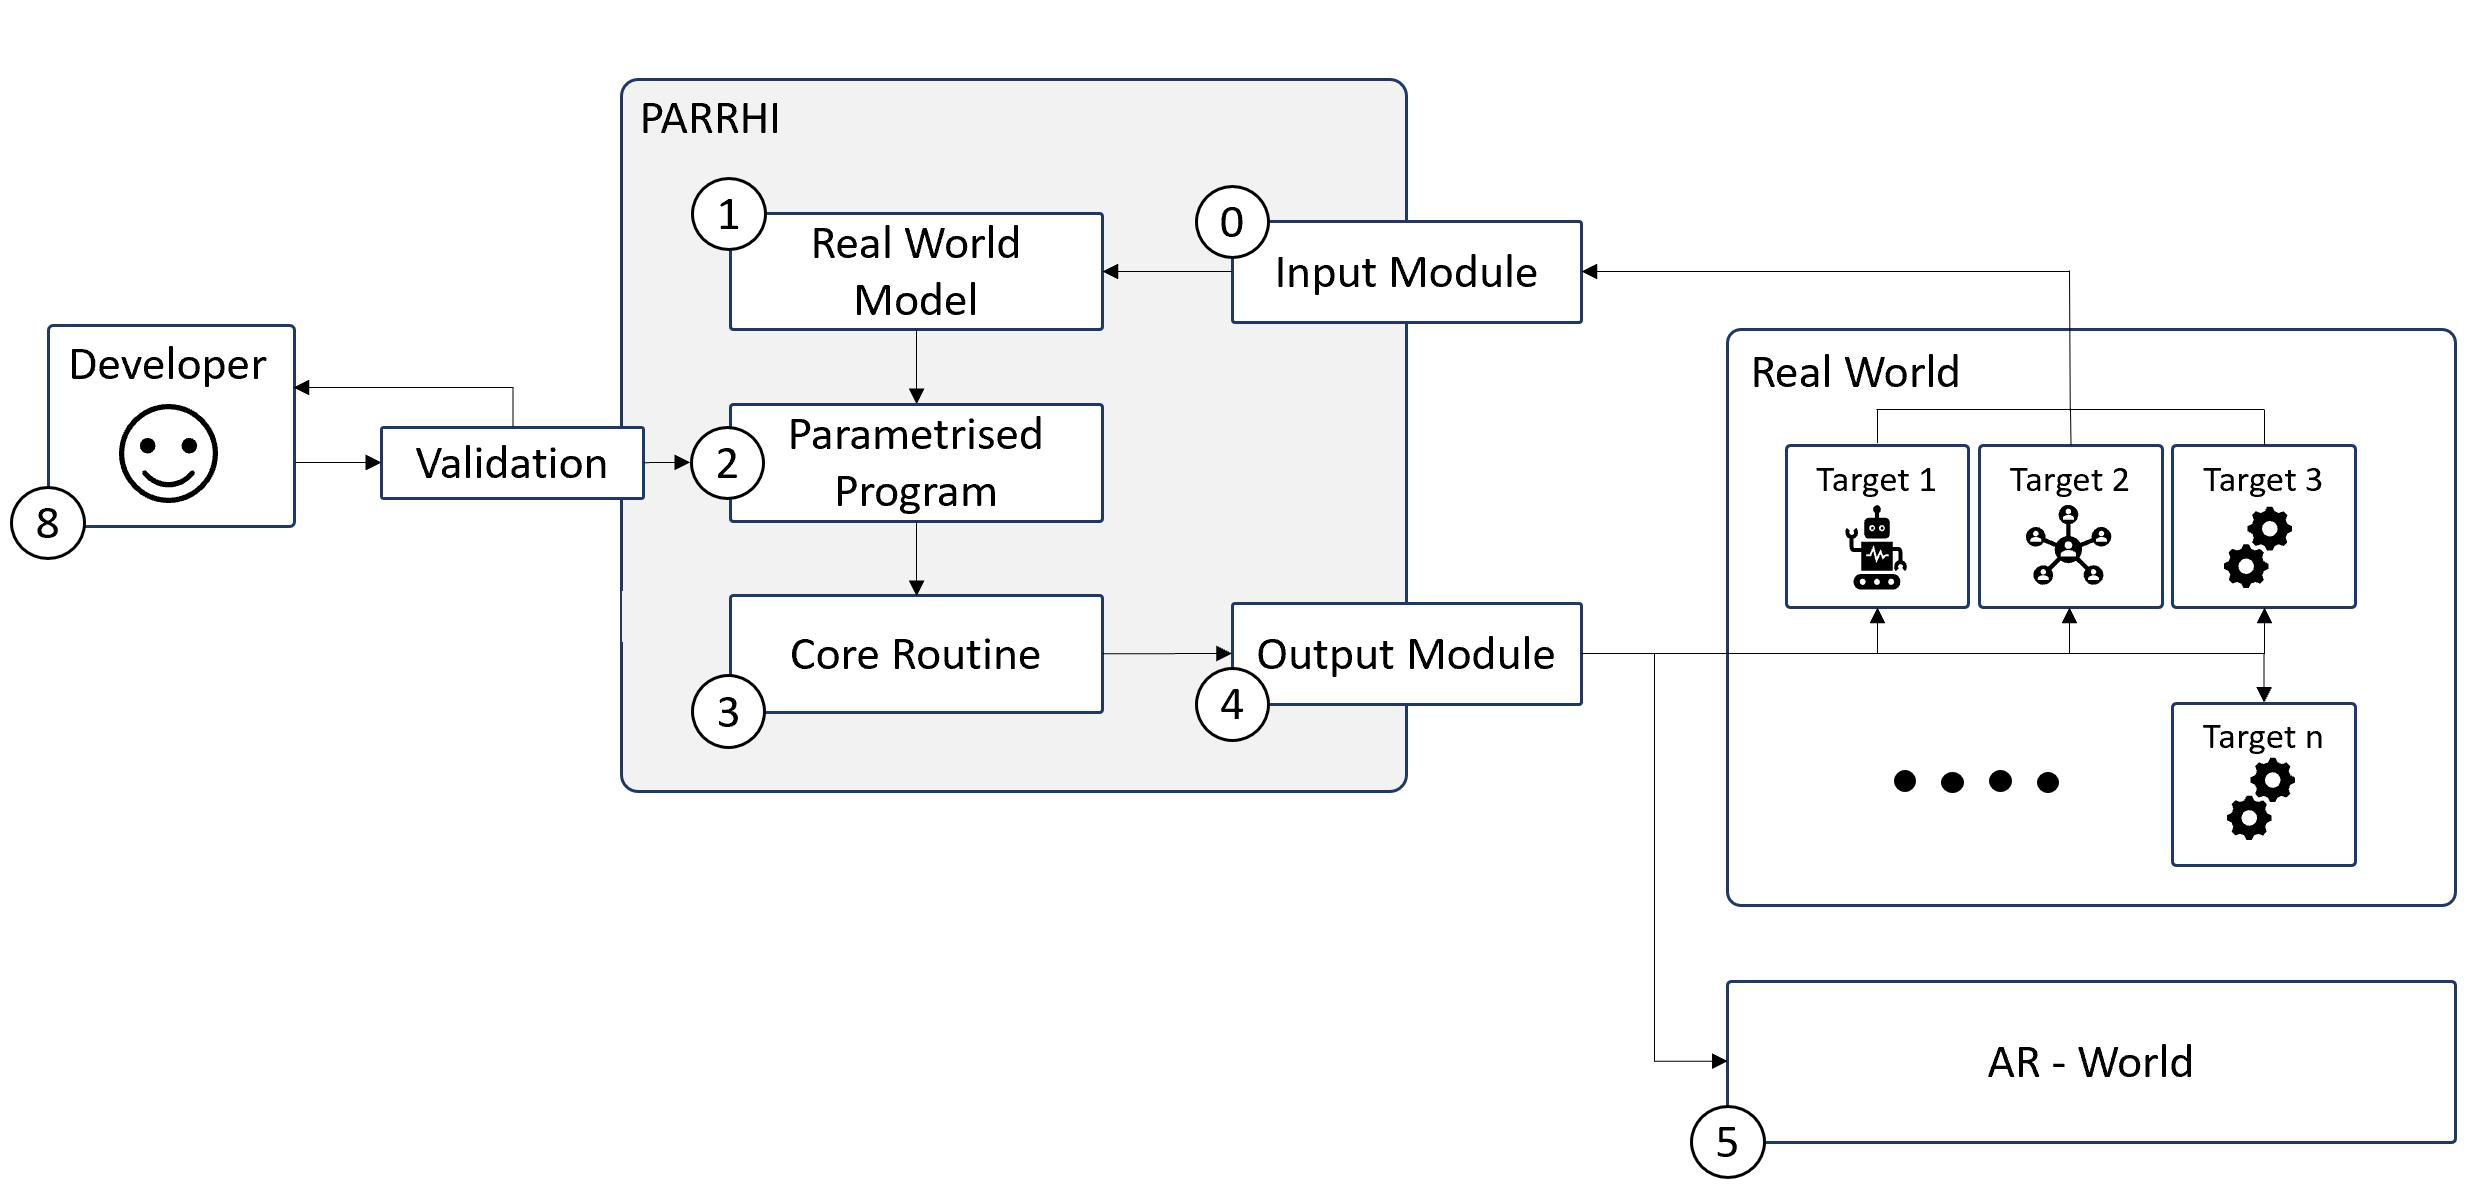
\includegraphics[width=0.8\linewidth]{Figures/FutureWork_ConceptV2}
	\caption[Future Work - Generalised Concept]{}
	\label{Fig:GeneralisedConcept}
\end{figure}













